\documentclass[11pt, a4paper]{article}\usepackage[]{graphicx}\usepackage[]{xcolor}
% maxwidth is the original width if it is less than linewidth
% otherwise use linewidth (to make sure the graphics do not exceed the margin)
\makeatletter
\def\maxwidth{ %
  \ifdim\Gin@nat@width>\linewidth
    \linewidth
  \else
    \Gin@nat@width
  \fi
}
\makeatother

\definecolor{fgcolor}{rgb}{0.345, 0.345, 0.345}
\newcommand{\hlnum}[1]{\textcolor[rgb]{0.686,0.059,0.569}{#1}}%
\newcommand{\hlsng}[1]{\textcolor[rgb]{0.192,0.494,0.8}{#1}}%
\newcommand{\hlcom}[1]{\textcolor[rgb]{0.678,0.584,0.686}{\textit{#1}}}%
\newcommand{\hlopt}[1]{\textcolor[rgb]{0,0,0}{#1}}%
\newcommand{\hldef}[1]{\textcolor[rgb]{0.345,0.345,0.345}{#1}}%
\newcommand{\hlkwa}[1]{\textcolor[rgb]{0.161,0.373,0.58}{\textbf{#1}}}%
\newcommand{\hlkwb}[1]{\textcolor[rgb]{0.69,0.353,0.396}{#1}}%
\newcommand{\hlkwc}[1]{\textcolor[rgb]{0.333,0.667,0.333}{#1}}%
\newcommand{\hlkwd}[1]{\textcolor[rgb]{0.737,0.353,0.396}{\textbf{#1}}}%
\let\hlipl\hlkwb

\usepackage{framed}
\makeatletter
\newenvironment{kframe}{%
 \def\at@end@of@kframe{}%
 \ifinner\ifhmode%
  \def\at@end@of@kframe{\end{minipage}}%
  \begin{minipage}{\columnwidth}%
 \fi\fi%
 \def\FrameCommand##1{\hskip\@totalleftmargin \hskip-\fboxsep
 \colorbox{shadecolor}{##1}\hskip-\fboxsep
     % There is no \\@totalrightmargin, so:
     \hskip-\linewidth \hskip-\@totalleftmargin \hskip\columnwidth}%
 \MakeFramed {\advance\hsize-\width
   \@totalleftmargin\z@ \linewidth\hsize
   \@setminipage}}%
 {\par\unskip\endMakeFramed%
 \at@end@of@kframe}
\makeatother

\definecolor{shadecolor}{rgb}{.97, .97, .97}
\definecolor{messagecolor}{rgb}{0, 0, 0}
\definecolor{warningcolor}{rgb}{1, 0, 1}
\definecolor{errorcolor}{rgb}{1, 0, 0}
\newenvironment{knitrout}{}{} % an empty environment to be redefined in TeX

\usepackage{alltt}

\usepackage[top = 0.75 in, bottom = 0.75 in, left = 1 in, right = 1 in ]{geometry}

\usepackage{amsmath, amssymb, amsfonts}
\usepackage{enumerate}
\usepackage{array}
\usepackage{multirow}
\usepackage{dingbat}
\usepackage{fontawesome5}
\usepackage{tasks}
\usepackage{bbding}
\usepackage{twemojis}
% how to use bull's eye ----- \scalebox{2.0}{\twemoji{bullseye}}
\usepackage{fontspec}
\usepackage{customdice}
% how to put dice face ------ \dice{2}

\title{MSMS 105 : Assignment 07}
\author{Ananda Biswas}
\date{\today}

\newfontface\myfont{Myfont1-Regular.ttf}[LetterSpace=0.05em]
% how to use ---- {\setlength{\spaceskip}{1em plus 0.5em minus 0.5em} \fontsize{17}{20}\myfont --write text here-- \par}

\newfontface\cbfont{CaveatBrush-Regular.ttf}
% how to use --- \myfont --write text here--
\IfFileExists{upquote.sty}{\usepackage{upquote}}{}
\begin{document}

\maketitle


\section*{\faArrowAltCircleRight[regular] \textcolor{blue}{Objective}}

Random number generation from $N(\mu, \sigma^2)$.




\section*{\faArrowAltCircleRight[regular] \textcolor{blue}{Theory}}

Let $U_1$ and $U_2$ be two iid $U(0, 1)$ variates. \\

Then,
\begin{align*}
X_1 &= \sqrt{-2 \,\, ln U_1} \,\, \cos (2 \pi U_2) \text{ and} \\
X_2 &= \sqrt{-2 \,\, ln U_1} \,\, \sin (2 \pi U_2)
\end{align*}

are independently distributed $N(0, 1)$ variates.


\section*{\faArrowAltCircleRight[regular] \textcolor{blue}{R Program}}

\begin{knitrout}
\definecolor{shadecolor}{rgb}{0.969, 0.969, 0.969}\color{fgcolor}\begin{kframe}
\begin{alltt}
\hldef{random_numbers} \hlkwb{<-} \hlkwa{function}\hldef{(}\hlkwc{n}\hldef{,} \hlkwc{seed} \hldef{=} \hlkwa{NULL}\hldef{)\{}
  \hldef{a} \hlkwb{<-} \hlnum{1103515245}
  \hldef{b} \hlkwb{<-} \hlnum{12345}
  \hldef{m} \hlkwb{<-} \hlnum{2}\hlopt{^}\hlnum{31} \hlopt{-} \hlnum{1}

  \hlkwa{if}\hldef{(}\hlkwd{is.null}\hldef{(seed))\{}
    \hldef{start_date} \hlkwb{<-} \hlkwd{as.POSIXct}\hldef{(}\hlsng{"2003-01-01 00:00:00"}\hldef{,} \hlkwc{tz} \hldef{=} \hlsng{"UTC"}\hldef{)}

    \hldef{current_date} \hlkwb{<-} \hlkwd{Sys.time}\hldef{()}

    \hldef{seed} \hlkwb{<-} \hlkwd{as.numeric}\hldef{(}\hlkwd{difftime}\hldef{(current_date, start_date,} \hlkwc{units} \hldef{=} \hlsng{"secs"}\hldef{))}
  \hldef{\}}

  \hldef{x} \hlkwb{<-} \hlkwd{c}\hldef{(seed)}

  \hlkwa{for} \hldef{(i} \hlkwa{in} \hlnum{2}\hlopt{:}\hldef{n) \{}
    \hldef{x[i]} \hlkwb{<-} \hldef{(a} \hlopt{*} \hldef{x[i}\hlopt{-}\hlnum{1}\hldef{]} \hlopt{+} \hldef{b)} \hlopt \hldef{m}
  \hldef{\}}

  \hlkwd{return}\hldef{(x)}
\hldef{\}}
\end{alltt}
\end{kframe}
\end{knitrout}

\begin{knitrout}
\definecolor{shadecolor}{rgb}{0.969, 0.969, 0.969}\color{fgcolor}\begin{kframe}
\begin{alltt}
\hldef{uniform_random_numbers} \hlkwb{<-} \hlkwa{function}\hldef{(}\hlkwc{n}\hldef{,} \hlkwc{seed} \hldef{=} \hlkwa{NULL}\hldef{)\{}
  \hlkwd{return}\hldef{(}\hlkwd{random_numbers}\hldef{(n, seed)} \hlopt{/} \hldef{(}\hlnum{2}\hlopt{^}\hlnum{31} \hlopt{-} \hlnum{1}\hldef{))}
\hldef{\}}
\end{alltt}
\end{kframe}
\end{knitrout}

\begin{knitrout}
\definecolor{shadecolor}{rgb}{0.969, 0.969, 0.969}\color{fgcolor}\begin{kframe}
\begin{alltt}
\hldef{normal_random_numbers} \hlkwb{<-} \hlkwa{function}\hldef{(}\hlkwc{n}\hldef{,} \hlkwc{mu}\hldef{,} \hlkwc{sigma}\hldef{,} \hlkwc{seed} \hldef{=} \hlkwa{NULL}\hldef{)\{}

  \hldef{u1} \hlkwb{<-} \hlkwd{uniform_random_numbers}\hldef{(n, seed)}
  \hldef{u2} \hlkwb{<-} \hlkwd{uniform_random_numbers}\hldef{(n, seed)}

  \hldef{x} \hlkwb{<-} \hlkwd{sqrt}\hldef{(}\hlopt{-}\hlnum{2} \hlopt{*} \hlkwd{log}\hldef{(u1))} \hlopt{*} \hlkwd{cos}\hldef{(}\hlnum{2} \hlopt{*} \hldef{pi} \hlopt{*} \hldef{u2)}

  \hldef{x} \hlkwb{<-} \hldef{mu} \hlopt{+} \hldef{sigma} \hlopt{*} \hldef{x}

  \hlkwd{return}\hldef{(x)}
\hldef{\}}
\end{alltt}
\end{kframe}
\end{knitrout}

\begin{knitrout}
\definecolor{shadecolor}{rgb}{0.969, 0.969, 0.969}\color{fgcolor}\begin{kframe}
\begin{alltt}
\hldef{size} \hlkwb{<-} \hlnum{10}
\hlkwd{normal_random_numbers}\hldef{(size,} \hlnum{1}\hldef{,} \hlnum{1}\hldef{)}
\end{alltt}
\begin{verbatim}
##  [1] 0.3370971 1.3099430 2.7139209 1.5683085 1.4309843 3.1268405 1.5811996
##  [8] 0.9139678 2.9715475 1.6044944
\end{verbatim}
\end{kframe}
\end{knitrout}


\newpage

\section*{\faArrowAltCircleRight[regular] \textcolor{blue}{Visualization}}



\begin{knitrout}
\definecolor{shadecolor}{rgb}{0.969, 0.969, 0.969}\color{fgcolor}\begin{kframe}
\begin{alltt}
\hldef{size} \hlkwb{<-} \hlnum{1000}
\hldef{normal_numbers} \hlkwb{<-} \hlkwd{data.frame}\hldef{(}\hlkwc{n} \hldef{=} \hlnum{1}\hlopt{:}\hldef{size,}
                          \hlkwc{num} \hldef{=} \hlkwd{normal_random_numbers}\hldef{(size,} \hlnum{1}\hldef{,} \hlnum{1}\hldef{))}
\end{alltt}
\end{kframe}
\end{knitrout}

\begin{knitrout}
\definecolor{shadecolor}{rgb}{0.969, 0.969, 0.969}\color{fgcolor}\begin{kframe}
\begin{alltt}
\hldef{normal_numbers} \hlopt
  \hlkwd{ggplot}\hldef{(}\hlkwd{aes}\hldef{(}\hlkwc{x} \hldef{= n,} \hlkwc{y} \hldef{= num))} \hlopt{+}
  \hlkwd{geom_point}\hldef{(}\hlkwc{size} \hldef{=} \hlnum{1.5}\hldef{,} \hlkwc{col} \hldef{=} \hlsng{"red"}\hldef{)} \hlopt{+}
  \hlkwd{geom_hline}\hldef{(}\hlkwc{yintercept} \hldef{=} \hlnum{1}\hldef{,} \hlkwc{col} \hldef{=} \hlsng{"blue"}\hldef{,} \hlkwc{linewidth} \hldef{=} \hlnum{1}\hldef{)} \hlopt{+}
  \hlkwd{labs}\hldef{(}\hlkwc{x} \hldef{=} \hlsng{"Index"}\hldef{,} \hlkwc{y} \hldef{=} \hlsng{"Random Numbers"}\hldef{,}
       \hlkwc{title} \hldef{=} \hlsng{"Random Numbers from N(1, 1)"}\hldef{)}
\end{alltt}
\end{kframe}
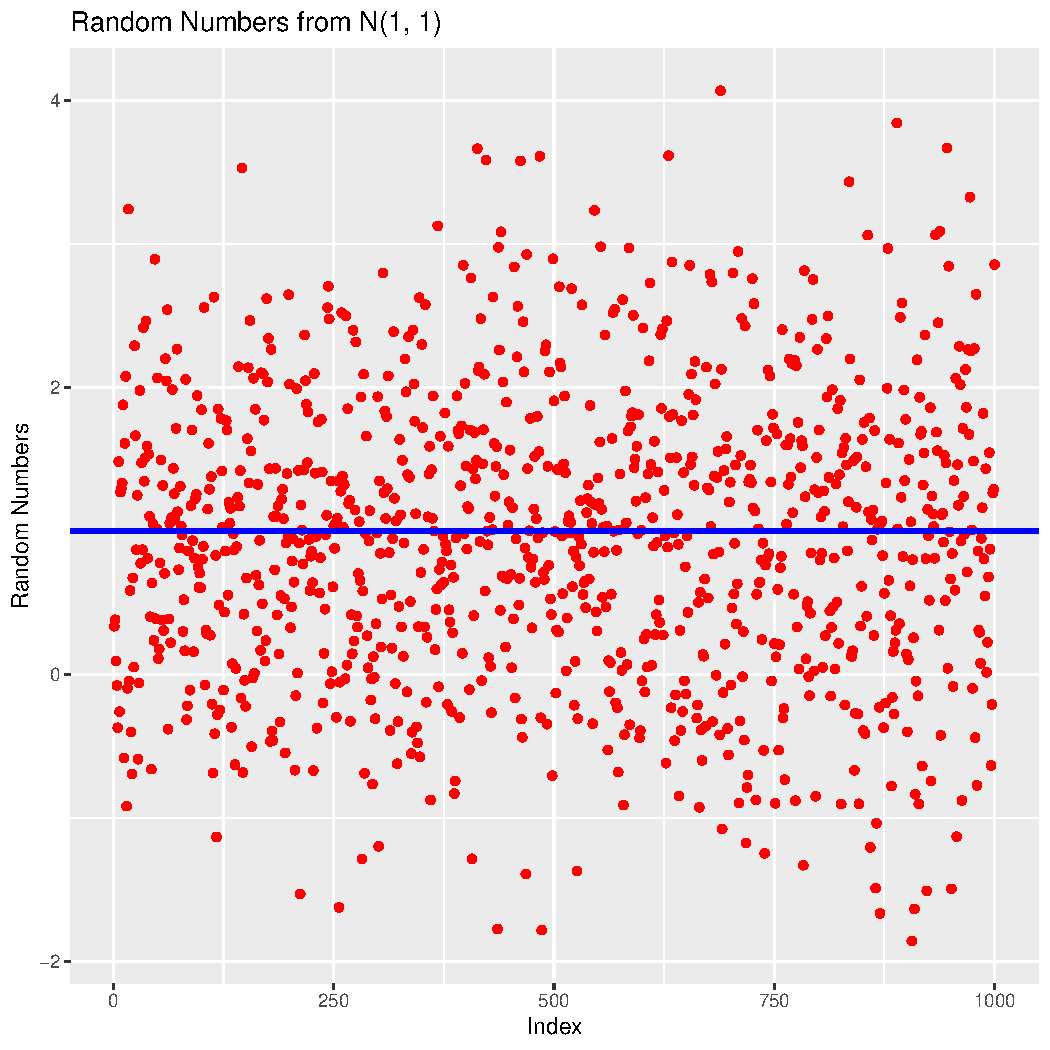
\includegraphics[width=\maxwidth]{figure/unnamed-chunk-7-1} 
\end{knitrout}

\section*{\faArrowAltCircleRight[regular] \textcolor{blue}{Conclusion}}

\smallpencil {\setlength{\spaceskip}{1em plus 0.5em minus 0.5em} \fontsize{17}{20}\myfont Scatteredness of the points mimics that of a $N(1, 1)$ Distribution. \par}

\end{document}
